\section{Ruteo interno y externo}
El problema de ruteo es como los switches y routers adquieren la información en sus tablas de forwarding.

Si bien los términos \textbf{tabla de forwarding} y \textbf{tabla de ruteo} son a veces usados indistintamente, haremos una distinción entre ellos aquí. La \textbf{tabla de forwarding} es usada cuando un paquete está siendo reenviado y por lo tanto debe contener suficiente información para realizar la función de forwarding. Esto significa que una fila en la tabla de forwarding contiene el mapeo de un prefijo de red a una interfaz de salida y alguna información MAC, como la dirección Ethernet del siguiente salto. La \textbf{tabla de ruteo}, por otro lado, es la tabla construida por los algoritmos de ruteo como un precursor para construir la tabla de forwarding. Generalmente contiene mapeos de prefijos de red a siguientes saltos. También puede contener información sobre cómo se aprendió esta información, para que el enrutador pueda decidir cuándo debe descartarla.

Los protocolos descritos en esta sección se conocen colectivamente como \textbf{protocolos de enrutamiento intradominio}, o Interior Gateway Protocols (IGP). Para comprender estos términos, debemos definir un dominio de enrutamiento: es una internet en la que todos los enrutadores están bajo el mismo control administrativo.

\subsection{La red como un grafo}
El ruteo es, en esencia, un problema de teoría de grafos. Los nodos del grafo pueden ser hosts, switches, routers o redes. Para nuestra discusión inicial, nos centraremos en el caso en que los nodos son enrutadores. Las aristas del grafo corresponden a los enlaces de red. Cada arista tiene un costo asociado, que da alguna indicación de la facilidad con la que se puede enviar tráfico a través de ese enlace.

Para resolver el problema de ruteo debemos encontrar el camino de menor costo entre dos nodos, donde el costo de un camino es igual a la suma de los costos de todas las aristas que componen el camino.

Los protocolos de ruteo proporcionan una forma distribuida y dinámica de resolver este problema en presencia de fallas de enlace y nodo y cambios en los costos de los enlaces.

Asumiendo que ya sabemos los costos de cada enlace vamos a ver dos algoritmos distribuidos que nos permiten crear la tabla de ruteo: \textbf{Distance Vector} y \textbf{Link State}.

\subsection{Distance Vector}
Cada nodo construye un vector que contiene las distancias (costos) a todos los otros nodos y distribuye ese vector a sus vecinos inmediatos. La suposición inicial para el ruteo vectorial de distancia es que cada nodo conoce el costo del enlace a cada uno de sus vecinos directamente conectados. Estos costos pueden ser provistos cuando el router es configurado por un administrador de red. Un enlace que está caído es asignado un costo infinito.

Inicialmente, cada nodo establece un costo de 1 a sus vecinos directamente conectados y \(\infty\) a todos los demás nodos.

En el siguiente paso, cada nodo envía un mensaje a sus vecinos directamente conectados indicando su lista personal de distancias.

Cuando un nodo recibe un vector de distancias, compara las distancias recibidas con las que tiene almacenadas en su tabla de ruteo. Si la distancia recibida es menor que la que tiene almacenada, la actualiza y envía su propio vector de distancias a sus vecinos.
\begin{figure}[H]
	\centering
	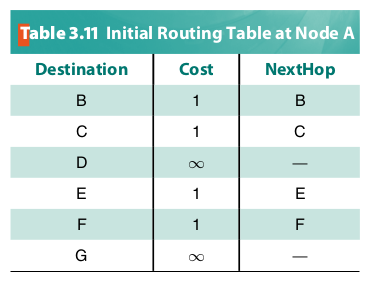
\includegraphics[width=0.5\textwidth
]{images/distance-vector-routing-table.png}
	\caption[Ejemplo tabla de ruteo]{Ejemplo tabla de ruteo}
	\label{fig:distance-vector-routing-table}
\end{figure}

En ausencia de cambios en la topología, solo se necesitan unos pocos intercambios de información entre vecinos antes de que cada nodo tenga una tabla de enrutamiento completa. El proceso de obtener información de enrutamiento consistente para todos los nodos se llama convergencia.

Los algoritmos distribuidos como este permiten que todos los nodos en la red se adapten automáticamente a los cambios en la topología de la misma. No se requiere intervención manual por parte de un administrador de red.

\subsubsection{Comportamiento ante fallas}
Hay dos circunstancias en las cuales un nodo dado decide enviar una actualización de enrutamiento a sus vecinos: 

\begin{itemize}
  \item Una \textbf{actualización periódica} se envía cada cierto tiempo, incluso si no ha cambiado nada. Esto sirve para que los otros nodos sepan que este nodo todavía está en funcionamiento. También se asegura de que sigan recibiendo información que puedan necesitar si sus rutas actuales se vuelven inviables. La frecuencia de estas actualizaciones periódicas varía de un protocolo a otro, pero generalmente está en el orden de varios segundos a varios minutos.
  \item Cuando un enlace o nodo falla (\textbf{triggered update}). Los nodos que notan esta situación primero envían nuevas listas de distancias a sus vecinos, y normalmente el sistema se estabiliza bastante rápido a un nuevo estado. 
\end{itemize}

Dependiendo el protocolo, la detección de una falla se puede dar de dos formas:
\begin{itemize}
  \item Un nodo prueba continuamente el enlace a otro nodo enviando un paquete de control y viendo si recibe un acuse de recibo.
  \item Un nodo determina que el enlace (o el nodo en el otro extremo del enlace) está inactivo si no recibe la actualización de enrutamiento periódica esperada durante los últimos ciclos de actualización.
\end{itemize}

\subsubsection{Conteo hasta el infinito}

Sucede cuando se cae un nodo o enlace y los nodos restantes no se dan cuenta de que el nodo o enlace ha fallado y hay nodos en la red que no alcanzan a enterarse de esto antes de que otro y deciden usarlos para crear el nuevo camino que los lleve al nodo caído. 
\begin{figure}[H]
	\centering
	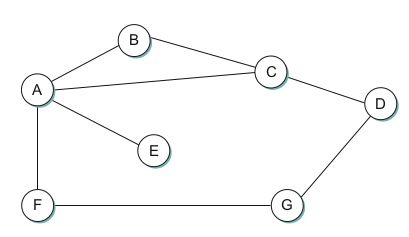
\includegraphics[width=0.5\textwidth
]{images/network-graph.png}
	\caption[Grafo de una red]{Grafo de una red}
	\label{fig:network-graph}
\end{figure}

Supongamos que se cae el enlace de \(A\) a \(E\) en la red mostrada arriba, supongamos se produce la ronda de periodic updates. Todos los nodos, envían su vector de distancias a sus vecinos. Puede suceder lo siguiente:
\begin{enumerate}
  \item  \(A\) anuncia una distancia de \(\infty\) a \(E\).
  \item \(B\) recibe de \(A\): \(\langle E,\infty\rangle\).
  \item \(B\) decide que a partir de ahora puede llegar a \(E\) usando \(C\) con una distancia de \(3\) y reenvía su vector de distancias antes de recibir el vector de distancias modificado de \(C\).
  \item \(A\) recibe el mensaje de \(B\) y decide que puede llegar a \(E\) usando \(B\) con una distancia de \(4\) y reenvía su vector de distancias.
  \item Cuando \(C\) reciba este paquete, sabe que puede usar \(A\) para recibir paquetes de \(E\) con una distancia de \(5\).
\end{enumerate}

Este ciclo se detiene solo cuando las distancias alcanzan algún número lo suficientemente grande como para considerarse infinito. Mientras tanto, ninguno de los nodos sabe realmente que \(E\) es inalcanzable, y las tablas de enrutamiento de la red no se estabilizan.

Hay varias soluciones parciales a este problema:
\begin{itemize}
  \item La primera es poner un número de distancia máximo pequeño como aproximación al infinito. Esto al menos limita la cantidad de tiempo que se tarda en contar al infinito. Por supuesto, también podría presentar un problema si nuestra red creciera hasta el punto en que algunos nodos estuvieran separados por más de la distancia máxima que habiamos definido.
  \item Otra técnica se llama \textbf{Split Horizon}: La idea es que cuando un nodo envía una actualización de enrutamiento a sus vecinos, no envía esas rutas que aprendió de cada vecino de vuelta a ese vecino. Por ejemplo, si \(B\) tiene la ruta \(\langle E, 2, A\rangle\) en su tabla, entonces sabe que debe haber aprendido esta ruta de \(A\), por lo que cada vez que \(B\) envía una actualización de enrutamiento a \(A\), no incluye la ruta \(\langle E, 2\rangle\) en esa actualización.
  \item Una variación más fuerte, llamada \textbf{Split Horizon with posion reverse}, vuelve a evniar la ruta \(A\) pero con una distancia de \(\infty\). Esto le dice a \(A\) que no puede llegar a \(E\) a través de \(B\).
\end{itemize}

El problema con estas técnicas que solo funcionan para loops que involucran dos nodos, se necesitan tomar decisiones más drásticas para loops más grandes. Se podría haber hecho que \(B\) y \(C\) esperen una cantidad determinada de tiempo antes de reenviar las nuevas rutas. Desafortunadamente, este enfoque retrasa la convergencia del protocolo; la velocidad de convergencia es una de las principales ventajas de su competidor: \textbf{Link-State Routing}.

\subsubsection*{Ruting Information Protocol (RIP)}
Uno de los protocolos de enrutamiento más utilizados en las redes IP es el Protocolo de Información de Enrutamiento (RIP).

En una internet, el objetivo de los enrutadores es aprender a reenviar paquetes a varias redes. Por lo tanto, en lugar de anunciar el costo de llegar a otros enrutadores, los enrutadores anuncian el costo de llegar a las redes.

RIP es una implementación bastante sencilla del algoritmo de Vector Distance Routing. Los enrutadores que ejecutan RIP envían sus anuncios cada 30 segundos.

Un enrutador también envía un mensaje de actualización cada vez que una actualización de otro enrutador hace que cambie su tabla de enrutamiento. Un punto de interés es que admite múltiples familias de direcciones, no solo IP. RIP versión 2 (RIPv2) también introdujo las máscaras de subred mientras que RIP versión 1 funcionaba con las direcciones de clase antigua de IP.

\subsection{Link State Routing}
Link State Routing es la segunda clase principal de protocolo de enrutamiento intradominio. Se supone que cada nodo es capaz de descubrir el estado del enlace a sus vecinos y el costo de cada enlace.

Cada nodo sabe cómo llegar a sus vecinos directamente conectados, si nos aseguramos de que la totalidad de este conocimiento se difunda a cada nodo entonces cada nodo tendrá suficiente conocimiento de la red para construir un mapa completo. Esta es una condición suficiente (aunque no necesaria) para encontrar el camino más corto a cualquier punto de la red. Los protocolos de link state routing se basan en dos mecanismos: la difusión confiable de la información de estado de enlace y el cálculo de rutas a partir de la suma de todo el conocimiento acumulado por este algoritmo.

\subsubsection{Reliable flooding}
La inundación confiable (reliable flooding) es el proceso de asegurarse de que todos los nodos que participan en el protocolo de enrutamiento obtengan una copia de la información de estado de enlace de todos los demás. Como sugiere el término inundación, la idea es que un nodo envíe su información de estado de enlace en todas sus conexiones directas; cada nodo que recibe esta información la reenvía en todas sus conexiones. Este proceso continúa hasta que la información ha llegado a todos los nodos de la red.

El paquete paquete de actualización que envían los nodos, también llamado paquete de estado de enlace (Link State Packet, LSP), contiene la siguiente información:

\begin{itemize}
  \item El ID del nodo que creó el LSP.
  \item Una lista de vecinos directamente conectados de ese nodo, con el costo del enlace a cada uno.
  \item Un número de secuencia
  \item Un tiempo de vida (Time To Live - TTL) para este paquete
\end{itemize}

Los primeros dos elementos son necesarios para permitir el cálculo de rutas; los dos últimos se utilizan para que el proceso de inundación del paquete a todos los nodos sea confiable. La confiabilidad incluye asegurarse de tener la copia más reciente de la información, ya que puede haber múltiples LSP contradictorios de un mismo nodo circulando en la red.

Veamos como el proceso de flooding: 
\begin{itemize}
  \item Supongamos que un nodo \(A\) crea un LSP y lo envía a todos sus vecinos.
  \item Un nodo \(B\) que recibe una copia de un LSP que se originó en \(A\).
  \item \(B\) compara el número de secuencia del LSP que acaba de recibir con el número de secuencia del LSP que ya tiene almacenado para \(A\). Si el nuevo LSP tiene un número de secuencia más grande, se asume que es el más reciente, y ese LSP se almacena, reemplazando al antiguo. Un número de secuencia más pequeño (o igual) implicaría un LSP más antiguo (o no más nuevo) que el almacenado, por lo que se descartaría y no sería necesario tomar más medidas.
  \item Si el LSP recibido fue el más nuevo, \(B\) envía una copia de ese LSP a todos sus vecinos, excepto al vecino del que acaba de recibir el LSP.
\end{itemize}

El hecho de que el LSP no se reenvíe de vuelta al nodo desde el que se recibió ayuda a poner fin a la inundación del mismo. Dado que \(B\) pasa el LSP a todos sus vecinos, que luego hacen lo mismo, la copia más reciente del LSP eventualmente llega a todos los nodos.

Al igual que en RIP, cada nodo genera LSPs bajo dos circunstancias:
\begin{itemize}
  \item La expiración de un LSP, debido a que su TTL ha llegado a cero.
  \item Un cambio en la topología de la red. Sin embargo, la única razón basada en la topología para que un nodo genere un LSP es si uno de sus enlaces conectados directamente o vecinos inmediatos ha fallado.
\end{itemize}

La falla de un enlace puede detectarse en algunos casos por el protocolo de capa de enlace. La desaparición de un vecino o la pérdida de conectividad con ese vecino se puede detectar mediante paquetes periódicos ``hello". Cada nodo envía estos a sus vecinos inmediatos a intervalos definidos. Si pasa suficiente tiempo sin recibir un ``hello" de un vecino, el enlace a ese vecino se declarará inactivo y se generará un nuevo LSP para reflejar este hecho.

\subsubsection{Consideraciones de diseño}
Uno de los objetivos de diseño más importantes de la inundación en este protocolo es que la información más reciente debe inundarse a todos los nodos lo más rápido posible, mientras que la información antigua debe eliminarse de la red. Además, es deseable minimizar la cantidad total de tráfico de enrutamiento que se envía por la red; después de todo, esto es solo una sobrecarga desde la perspectiva de aquellos que realmente usan la red para sus aplicaciones. 

Una forma facil de reducir el overhead es generar LSPs solo cuando es necesario. Esto puede hacerse usando TTLs muy largos, a menudo del orden de horas. Dado que el protocolo de inundación es realmente confiable cuando cambia la topología, es seguro asumir que no es necesario emitir mensajes de que algo ha cambiado.

El algoritmo de enrutamiento de estado de enlace tiene muchas propiedades agradables: se ha demostrado que se estabiliza rápidamente, no genera mucho tráfico y responde rápidamente a los cambios de topología o fallas de los nodos. Por otro lado, la cantidad de información almacenada en cada nodo (un LSP para cada nodo en la red) puede ser bastante grande.

\subsubsection{Número de secuencia}
Cada vez que un nodo genera un nuevo LSP, lo incrementa en 1. A diferencia de la mayoría de los números de secuencia utilizados en otros protocolos, no se espera que estos se reseteen, por lo que el campo debe ser bastante grande (digamos, 64 bits). 

Si un nodo se apaga y luego vuelve a encenderse, comienza con un número de secuencia de 0. Si el nodo estuvo inactivo durante mucho tiempo, todos los LSP antiguos para ese nodo habrán expirado; de lo contrario, eventualmente recibirá una copia de su propio LSP con un número de secuencia más alto, que luego puede incrementar y usar como su propio número de secuencia. Esto asegurará que su nuevo LSP reemplace cualquiera de sus viejos LSP que hayan quedado desde antes de que el nodo se apagara.

\subsubsection{Time To Live}
Se usa para asegurarse de que la información de estado de enlace antigua se elimine eventualmente de la red. Un nodo siempre decrementa el TTL de un LSP recién recibido antes de inundarlo a sus vecinos. También "envejece" el LSP mientras se almacena en el nodo. Cuando el TTL llega a 0, el nodo vuelve a inundar el LSP con un TTL de 0, que es interpretado por todos los nodos de la red como una señal para eliminar ese LSP.

\subsubsection{Calculo de rutas}
Una vez que un nodo determinado tiene una copia del LSP de todos los nodos de la red, puede calcular un mapa completo para la topología de la red, y a partir de este mapa puede decidir la mejor ruta para cada destino.

En la práctica, cada switch calcula su tabla de enrutamiento directamente a partir de los LSP que ha recopilado utilizando una versión del algoritmo de Dijkstra llamado algoritmo de \textbf{forward searching}. Específicamente, cada switch mantiene dos listas, conocidas como \texttt{Tentative} y \texttt{Confirmed}. Cada una de estas listas contiene un conjunto de entradas de la forma \\ \(\langle \texttt{Destino}, \texttt{Costo}, \texttt{NextHop}\rangle\). El algoritmo funciona de la siguiente manera:
\begin{enumerate}
  \item Se inicializa la lista \texttt{Confirmed} con una entrada para el propio nodo; esta entrada tiene un costo de 0.
  \item Para el nodo recién agregado a la lista \texttt{Confirmed} en el paso anterior,  se selecciona su LSP y lo marcamos como \texttt{Next}.
  \item Para cada vecino (\texttt{Neighbor}) de \texttt{Next}, se calcula el costo (\textbf{Costo}) para llegar a este Vecino como la suma del costo desde mí mismo hasta \texttt{Next} y desde \texttt{Next} hasta \texttt{Neighbor}.
  \begin{enumerate}
    \item Si \texttt{Neighbor} no está actualmente en la lista \texttt{Confirmed}  ni en la lista \texttt{Tentative}, agregue \(\langle\texttt{Vecino}, \texttt{Costo}, \texttt{NextHop}\rangle\) a la lista \texttt{Tentative}, donde \texttt{NextHop} es el nodo al que necesito ir para llegar a \texttt{Next}.
    \item Si \texttt{Neighbor} está actualmente en la lista \texttt{Tentative}, y el \texttt{Costo} es menor que el costo actualmente listado para \texttt{Neighbor}, reemplace la entrada actual con \\ \(\langle\texttt{Neighbor}, \texttt{Costo}, \texttt{NextHop}\rangle\), donde \texttt{NextHop} es el nodo al que necesito ir para llegar a \texttt{Next}.
  \end{enumerate}
  \item Si \texttt{Tentative} está vacía, ya están todas las rutas calculadas. De lo contrario, se elije la entrada con el costo más bajo, se la mueve \texttt{Confirmed} y se vuelve a hacer todo el proceso desde el paso 2.
\end{enumerate}

\subsubsection{Open Shortest Path First Protocol (OSPF)}
OSPF agrega una cantidad considerable de características al algoritmo básico de link-state descrito anteriormente:

\begin{itemize}
  \item \textbf{Autenticación de mensajes de enrutamiento}: una característica de los algoritmos de enrutamiento distribuido es que dispersan información de un nodo a muchos, y toda la red puede verse afectada por la información incorrecta de un nodo. Por esta razón, es una buena idea asegurarse de que todos los nodos que participan en el protocolo puedan confiar en ellos. La autenticación de mensajes de enrutamiento ayuda a lograr esto.
  \item \textbf{Jerarquía}: Es una de las herramientas fundamentales utilizadas para hacer que los sistemas sean más escalables. OSPF introduce otra capa de jerarquía en el enrutamiento al permitir que un dominio se divida en áreas. Esto significa que un enrutador dentro de un dominio no necesariamente necesita saber cómo llegar a cada red dentro de ese dominio, puede ser capaz de salir adelante sabiendo cómo llegar a la zona correcta. Por lo tanto, hay una reducción en la cantidad de información que debe transmitirse y almacenarse en cada nodo.
  \item \textbf{Balanceo de carga}: OSPF permite que varias rutas al mismo lugar se asignen el mismo costo y hará que el tráfico se distribuya uniformemente entre ellas, lo que permite un mejor uso de la capacidad de red disponible.
  \item Todo el paquete, excepto los datos de autenticación, está protegido por una suma de comprobación de 16 bits utilizando el mismo algoritmo que la cabecera IP.
  \item 
\end{itemize}

De los cinco tipos de mensajes OSPF, el tipo 1 es el mensaje "hola", que un enrutador envía a sus pares para notificarles que todavía está vivo y conectado como se describe anteriormente. Los tipos restantes se utilizan para solicitar, enviar y confirmar la recepción de mensajes de estado de enlace. El bloque de construcción básico de los mensajes de estado de enlace en OSPF es el anuncio de estado de enlace (Link Stata advertisement - LSA). Un mensaje puede llegar a contener varios LSA.

Específicamente, un enrutador que ejecuta OSPF puede generar LSPs que anuncian una o más de las redes que están directamente conectadas a ese enrutador. Además, un enrutador que está conectado a otro enrutador por algún enlace debe anunciar el costo de llegar a ese enrutador a través del enlace. Estos dos tipos de anuncios son necesarios para permitir que todos los enrutadores en un dominio determinen el costo de llegar a todas las redes en ese dominio y el siguiente salto apropiado para cada red.

\subsection{Métricas}
Una de las métricas más basicas, que es bastante razonable y muy simple, es asignar un costo de 1 a todos los enlaces: la ruta de menor costo será la que tenga menos saltos. Sin embargo, dicho enfoque tiene varias desventajas:
\begin{itemize}
  \item No distingue entre enlaces en función de la latencia,
  \item No distingue entre rutas en función de la capacidad,
  \item No distingue entre enlaces en función de su carga actual, lo que hace imposible evitarlos si están sobrecargados.
\end{itemize}

\subsubsection{ARPANET}
La métrica de enrutamiento original de ARPANET medía la cantidad de paquetes que se encolaban esperando ser transmitidos en cada enlace. Sin embargo, dado que la longitud de la cola es una medida artificial de la carga, cuando un enlace tiene un costo demasiado alto, los paquetes se terminan enviando hacia la cola más corta en lugar de hacia el destino.

\subsubsection{ARPANET v2}
Una segunda versión del algoritmo de ruteo ARPANET, a veces llamado el nuevo mecanismo de ruteo, tuvo en cuenta tanto el ancho de banda del enlace como la latencia y utilizó el retraso, en lugar de la longitud de la cola, como medida de carga. Esto se hizo de la siguiente manera. Primero, cada paquete entrante se marca con la hora de llegada al enrutador (\(ArrivalTime\)) y se registra su hora de salida del enrutador (\(DepartTime\)). En segundo lugar, cuando se recibió el ACK de nivel de enlace desde el otro lado, el nodo calculó el retraso para ese paquete como 

\[Delay = (DepartTime - ArrivalTime) + TransmissionTime + Latency\]

donde \(TransmissionTime\) y \(Latency\) se definieron estáticamente para el enlace y representan el ancho de banda y la latencia del mismo, respectivamente.

Si el ACK no llegó, sino que en su lugar el paquete agotó el tiempo de espera, entonces \(DepartTime\) se restablece al momento en que se retransmitió el paquete. En este caso, \(DepartTime - ArrivalTime\) captura la confiabilidad del enlace: cuanto más frecuente sea la retransmisión de paquetes, menos confiable será el enlace y más querremos evitarlo. Finalmente, el peso asignado a cada enlace se deriva del retraso promedio experimentado por los paquetes enviados recientemente a través de ese enlace.

Sin embargo, bajo una carga pesada, un enlace congestionado comienza a anunciar un costo muy alto. Esto causa que todo el tráfico se moviera fuera de ese enlace, dejándolo inactivo, por lo que luego anunciaría un costo bajo, atrayendo de vuelta todo el tráfico, y así sucesivamente. El efecto de esta inestabilidad es que, bajo una carga pesada, muchos enlaces pasarían mucho tiempo inactivos, que es lo último que desea bajo una carga pesada.

\subsubsection{Revised ARPANET Routing Metric}
Un tercer enfoque, llamado "métrica de enrutamiento ARPANET revisada", abordó estos problemas. Los principales cambios fueron comprimir el rango dinámico de la métrica considerablemente, tener en cuenta el tipo de enlace y suavizar la variación de la métrica con el tiempo.

La suavización se logró usando los siguientes mecanismos:
\begin{itemize}
  \item La medición del retraso se transformó en una utilización del enlace, y este número se promedió con la última utilización informada para suprimir los cambios repentinos.
  \item Se impuso un límite estricto sobre cuánto podría cambiar la métrica de un ciclo de medición al siguiente. Al suavizar los cambios en el costo, la probabilidad de que todos los nodos abandonen una ruta a la vez se reduce en gran medida.
\end{itemize} 